\documentclass[eng,printmode]{mgr}
%opcje klasy dokumentu mgr.cls zostały opisane w dołączonej instrukcji

%poniżej deklaracje użycia pakietów, usunąć to co jest niepotrzebne
\usepackage{polski} %przydatne podczas składania dokumentów w j. polskim
%\usepackage[polish]{babel}%alternatywnie do pakietu polski, wybrać jeden z nich
\usepackage[utf8x]{inputenc} %kodowanie znaków, zależne od systemu
\usepackage[T1]{fontenc} %poprawne składanie polskich czcionek

%pakiety do grafiki
\usepackage{graphicx}
\usepackage{subfigure}
\usepackage{psfrag}
\usepackage{epstopdf}

\usepackage{indentfirst}
%pozycjonowanie grafiki
\usepackage{float}
\graphicspath{ {figures/} }

%pakiety dodające dużo dodatkowych poleceń matematycznych
\usepackage{amsmath}
\usepackage{amsfonts}

%pakiety wspomagające i poprawiające składanie tabel
\usepackage{supertabular}
\usepackage{array}
\usepackage{tabularx}
\usepackage{hhline}

%pakiet wypisujący na marginesie etykiety równań i rysunków zdefiniowanych przez \label{}, chcąc wygenerować finalną wersję dokumentu wystarczy usunąć poniższą linię
\usepackage{showlabels}

%pozostałe ustawienia
\usepackage[hidelinks,pagebackref=true,backref=false]{hyperref}
%\usepackage{lscape}
%\usepackage{pdflscape}
\usepackage{rotating}
\usepackage{changepage}

\usepackage{booktabs}

\topmargin -9mm

%ustawienia spisu treści
%\setcounter{tocdepth}{3}
%\setcounter{secnumdepth}{3}

%dane do złożenia strony tytułowej
\title{Badanie czasu pracy}
\engtitle{Work time guardian}
\author{Mikołaj Jermakowicz, Kamil Machnicki}
\supervisor{dr inż. Marek Woda}
%\date{2008} %standardowo u dołu strony tytułowej umieszczany jest bieżący rok, to polecenie pozwala wstawić dowolny rok

\field{Informatyka (INF)}
\specialisation{Inżynieria Internetowa (INT)}

\makeatletter
\hypersetup{
	pdfstartview={XYZ null null 1.00},
	pdfpagemode=UseNone,
	pdfauthor={\@author},
	pdftitle={\@title},
	pdfsubject={\@naglowek},
	pdfcreator={pdf\LaTeX}, 
	pdfproducer={TeXstudio}
}
\makeatother

\let\origappendix\appendix % save the existing appendix command
\renewcommand\appendix{\clearpage\pagenumbering{Roman}\origappendix}
\usepackage{etoolbox}
\apptocmd{\thebibliography}{\raggedright}{}{}

%\usepackage{spacje}

%definicje własnych poleceń
%\newcommand{\R}{I\!\!R} %symbol liczb rzeczywistych, działa tylko w trybie matematycznym
%\newtheorem{theorem}{Twierdzenie}[section] %nowe otoczenie do składania twierdzeń
\begin{document}
\bibliographystyle{plabbrv} %tylko gdy używamy BibTeXa, ustawia polski styl bibliografii

\maketitle %polecenie generujące stronę tytułową

\tableofcontents %spis treści

\chapter{Wstęp}

Jako zaliczenie kursu Zastosowania Systemów Wbudowanych należało zrealizować wybrany przez grupę projekt, dotyczący układów wbudowanych. Pracę wykonać można było wykorzystując platformy Raspberry Pi, Arduino, bądź Beagleboard. Przez naszą grupę wybrany został temat \emph{Badanie czasu pracy}, który zrealizowany został na płytce Raspberry Pi.

\section{Cel i zakres pracy}

Celem wybranego tematu było stworzenie projektu, który badałby godziny pracy pracowników danej placówki. Każdy pracownik przy wejściu oraz wyjściu odbijałby się przypisaną do siebie kartą, a system zliczałby godziny spędzone tego dnia i przedstawiał je w wygodnej formie dla administratora. Administrator mógłby dodawać pracowników oraz przypisać kartę do pracownika. W przypadku, gdy uprawniony użytkownik (taki, który znajduje się w bazie) odbije się w systemie, system poinformuje go o tym w sposób wizualny, a administrator będzie mógł zobaczyć w panelu dane pracownika i godzinę odbicia. W przypadku, gdy odbijana karta nie jest przypisana do żadnego pracownika, system w sposób wizualny zaalarmuje o tym.

\section{Funkcjonalności}

Lista funkcjonalności wymaganych do zrealizowania projektu:

\begin{itemize}
  \item Rozpoznawanie pracownika na podstawie odczytu z karty.
  \item Zapis godziny wejścia i wyjścia pracownika.
  \item Prezentacja danych zebranych w bazie danych.
  \item Sygnalizacja przepuszczenia pracownika i błędnej karty.
  \item Panel wyświetlania pracowników i godziny ich pracy.
  \item Panel dodawania nowych pracowników i przypisywania do nich karty.
\end{itemize}

\section{Moduły}

Aby zrealizować projekt, został on podzielony na dwa moduły:

\begin{enumerate}
  \item \textbf{Sterownik} - moduł obsługujący wczytywanie karty i zapisywanie danych do bazy, a także informowanie użytkownika o pomyślnej bądź niepomyślnej autoryzacji.
  \item \textbf{Aplikacja} - panel administratora, gdzie wyświetlane są godziny pracy pracowników oraz gdzie można zarządzać pracownikami i przypisywać do nich karty.
\end{enumerate}
\chapter{Sterownik}
\chapter{Aplikacja}
\section{Program prezentacji danych}
Aplikacja została wykonana z myślą o pracodawcy, który chciałby mieć podgląd obecnych pracowników w biurze, oraz podsumowanie przepracowanego czasu dla poszczególnego pracownika.

Aplikacja składa się z kilku modułów:

\begin{enumerate}
  \item \texttt{main.py} - główny moduł systemu, odpowiada za uruchomienie aplikacji.
  \item \texttt{workingTimeDialog.py} - obsługa bazy danych i zapytań użytkownika.
  \item \texttt{uiWorkingTime.py} - moduł konfigurujący gradiczny interfejs.
\end{enumerate}

Program uruchamia się wpisując w konsoli:

\begin{verbatim}
python3 main.py
\end{verbatim}
\newpage
\subsection{Podgląd obecnych pracowników}
W tej części programu można podejżeć obecnych pracowników ich imię, nazwisko oraz czas przybycia.
Widok odświeża się do pół sekundy.

\begin{figure}[h!]
	\centering
	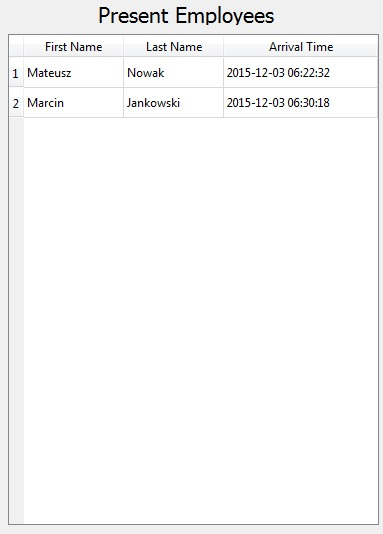
\includegraphics[width=0.37\linewidth]{img/present_employees.jpg}
	\label{fig:present_employees}
	\caption[Obecni pracownicy]{Obecni pracownicy}
\end{figure}

\subsection{Podgląd prepracowanego czasu pracowników}
Podgląd umożliwia wybrania przedziału czasu. Nastepnie wyświetli się imie, nazwisko oraz przepracowany czas.
\begin{figure}[h!]
	\centering
	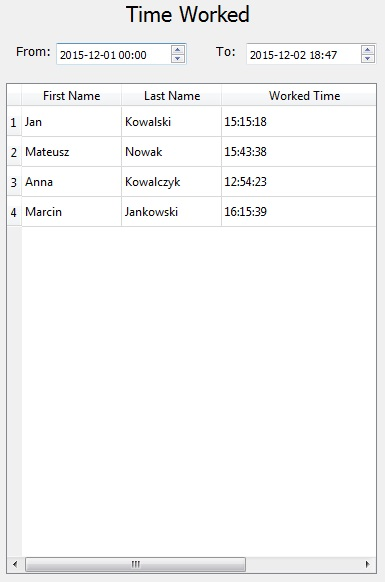
\includegraphics[width=0.37\linewidth]{img/time_worked.jpg}
	\label{fig:time_worked}
	\caption[Przepracowany czas]{Przepracowany czas}
\end{figure}
\newpage
\subsection{Dodawanie pracowników}
Ta część programu pozwala na dodawanie użytkowników. Wymagane są wszystkie pola do wpsiania.
Należy podać: Imię, Nazwisko, id taga rfid. email oraz hasło do systemu.
\begin{figure}[h!]
	\centering
	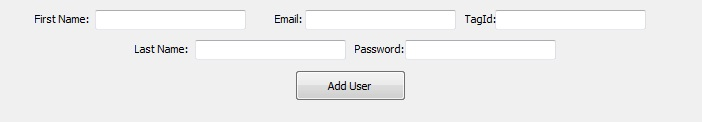
\includegraphics[width=0.80\linewidth]{img/add_user.jpg}
	\label{fig:add_user}
	\caption[Dodaj pracownika]{Dodaj pracownika}
\end{figure}

\section{Technologie}
Wykorzystane technologie:
\begin{itemize}
\item Python3.4 - Język programowania, w którym została wykonana aplikacja.
\item PyQt5 - Biblioteka języka python do interfejsu graficznego.
\item psycopg2 - Biblioteka języka python do komunikacji z bazą danych PostgreSQL
\item PostgreSQL - Baza danych.
\item Vagrant - Środowisko do przygotowania maszyn wirtualnych.
\item Raspbian - Dystrybujca linuxa przygotowanego dla RPi na podstawie dystrybucji Debian.
\end{itemize}
\section{Przygotowanie środowiska}
Aby uruchomić program prezentacji danych potrzeba zainstalować interpreter Python3.4, oraz biblioteki PyQt5, psycopq2. Program używa danych przetrzymywanych w bazie danych PostgreSQL.
\section{Baza Danych}
Baza danych składa się z dwóch tabel, Pracowników oraz przejść. Do każdego pracownika może być przypisane wiele przejść.

\begin{figure}[h!]
	\centering
	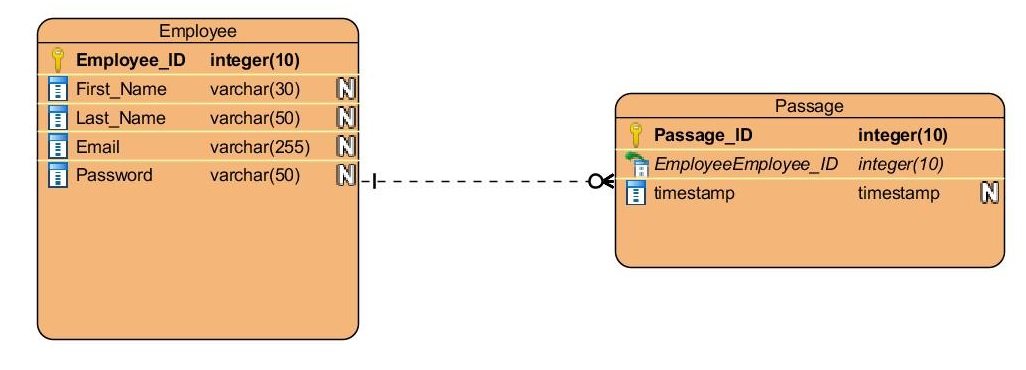
\includegraphics[width=\linewidth]{img/ERD_screen.jpg}
	\label{fig:ERD}
	\caption[Diagram ERD]{Diagram ERD}
\end{figure}
Możliwe jest ustawinie bazy danych na dowolonym urządzeniu. Takie rozwiązanie było niezbedne ze względu na to, że posiadaliśmy tylko jeden komputer RPi. Aplikacja prezentacji danych, komunikuje się wyłącznie z bazą danych, więc możliwe było tworzenie aplikacji bez komputera RPi.
\subsection{Baza danych na maszynie wirtualnej}
W ramach projektu został przygotowany plik konfiguracyjny maszyny\\ (github:/database/Vagrantfile). Aby wygenerować maszynę wirtualną potrzebny jest program Vagrant. Uruchomienie skonfigurowanej maszyny wirtualenej, polega na wejściu do katalogu z plikiem konfigurayjnym i wywołaniem komędy "vagrant up". Następnie trzeba przekazać port 5432 bazy danych z maszyny wirtualnej do systemu operacyjnnego na ip 127.0.0.1, w projekcie wykorzystywany był do tego program putty.
Dane logowania do maszyny wirtualnej to: użytkownik - vagrant, hasło - vagrant.
\subsection{Baza dnych na Raspberry Pi}
Do pracy na RPi Wybraliśmy dystrybucje linuxa Raspbian.
Aby skonfigurować bazę danych na Raspberry Pi należy wykonać następujące komendy:
\lstset{language=bash, breaklines=true}
\begin{lstlisting}
apt-get update
apt-get install postgresql postgresql-contrib postgis gpsbabel git libsqlite3-dev libreadline-dev libpq-dev libbz2-dev zlib1g-dev libpqxx-dev libzip-dev -y
echo -ne "alamakota\nalamakota" | su - postgres -c 'createuser -P -e wbudowane'
su - postgres -c 'createdb -e -O wbudowane wbudowane'
su - postgres -c 'psql wbudowane < /vagrant/czaspracyBD.sql'
su - postgres -c 'psql wbudowane -c "GRANT ALL ON TABLE Employee TO wbudowane;"'
su - postgres -c 'psql wbudowane -c "GRANT ALL ON TABLE Passage TO wbudowane;"'
su - postgres -c 'psql wbudowane -c "GRANT USAGE, SELECT ON ALL SEQUENCES IN SCHEMA public to wbudowane;"'
\end{lstlisting}




\chapter{Podsumowanie}

\nocite{*}
\newpage
\phantomsection
\addcontentsline{toc}{chapter}{\bibname}
\bibliography{bibliografia}

\newpage
\phantomsection
\addcontentsline{toc}{chapter}{\listfigurename}
\listoffigures

\newpage
\phantomsection
\addcontentsline{toc}{chapter}{\listtablename}
\listoftables

\end{document}

